\section{Finalization}
\label{sec:finalization}

\nemquote{%
And it feels like, finally.
}{Patrick Ness}

The CAP Theorem posits that, in the presence of a network failure or partition,
a distributed system must choose either \emph{consistency} or \emph{availability}.

In a consistent system, requests sent to two nodes will always return the same value.
If the value is not globally agreed upon, the request will fail.
This ensures that all clients have a uniform view of the system.
BFT systems typically choose consistency and risk network stalls.
A naive consistent system could require all stakeholders to vote on each block
and only allow the next block when $\frac{2}{3}$ of stakeholders approve.
If stakeholders fail to vote promptly, there could be a delay in block production.

In an available system, requests sent to two nodes will always return a value immediately.
The returned values can be different, so different clients could have different views of the system.
PoW and NXT-style PoS systems typically chose availability and eventual consensus.
They risk propagating different (potentially unresolvable) views of the system.
Available PoW-like systems, like Bitcoin, have a simple fork rule that chooses the chain with the most work.
If the network is split into partitions with equal hash power, all partitions will proceed independently without knowing they’re partitioned.
When they are eventually reconnected, there will be an expensive (and potentially deep) fork resolution.

\codenamespace always prefers availability over consistency, but it optionally supports the use of a finality gadget on top of its native consensus \nemrefparens{sec:consensus}.
This gadget introduces a BFT-inspired voting system that is orthogonal to block production and block consensus.
As a result of its optionality, \codenamespace is able to support networks that use either deterministic finalization (when the gadget is enabled) or probabilistic finalization (when the gadget is disabled).
The gadget is automatically enabled when \nemsetting{node}{maxRollbackBlocks} is zero\footnote{
	The finalization extension must also be enabled.
}.

The gadget approach is modeled after GRANDPA \cite{Stewart2020grandpa} used by Polkadot.
GRANDPA, in turn, in influenced by CASPER \cite{CasperFfg}, which itself is influenced by PBFT \cite{Pbft1999}.
Traditionally, PBFT uses three types of messages: pre-prepare, prepare and commit.
Pre-prepare messages, which are used to start rounds, are not used in \codenamespace.
Instead, elapsed network time \nemrefparens{sec:timesync} is used to start rounds.
Prepare and commit messages in PBFT roughly correspond to prevote and precommit messages in \codenamespace.

\subsection{High Level Overview}

Block finalization is a complicated process that involves two types of messages: prevotes and precommits.
At the beginning of a round, each voter only knows the blocks stored in its local chain.
No voter knows the blocks stored in the chains of any other voter.
Consequently, it is impossible for a voter to know which of its blocks will receive a supermajority of votes and be finalized ahead of time.

To illustrate the general procedure of finalization, consider a network composed of three equally weighted voters.
A supermajority requires at least two of the three voters to vote for the same hash.
$F$ refers to the last finalized block.

\begin{figure}[H]
	\nemcenter{
		\begin{tikzpicture}[every node/.style = {shape=rectangle, rounded corners, draw, align=center}]
			\tikzset{
				fill fraction/.style n args={3}{
					path picture={
						\fill[#1]
							($(path picture bounding box.south west)!#2!(path picture bounding box.south east)$)
							rectangle
							($(path picture bounding box.north west)!#3!(path picture bounding box.north east)$);
					}
				}
			}

			\tikzset{ vote1/.style = { fill fraction={red!25}{0.00}{0.33} } }
			\tikzset{ vote2/.style = { fill fraction={green!25}{0.33}{0.66} } }
			\tikzset{ vote3/.style = { fill fraction={blue!25}{0.66}{0.99} } }

			\tikzset{ vote23/.style = {
					path picture={
						\fill[green!25]
							($(path picture bounding box.south west)!0.33!(path picture bounding box.south east)$)
							rectangle
							($(path picture bounding box.north west)!0.66!(path picture bounding box.north east)$);
						\fill[blue!25]
							($(path picture bounding box.south west)!0.66!(path picture bounding box.south east)$)
							rectangle
							($(path picture bounding box.north west)!0.99!(path picture bounding box.north east)$);
					}
				}
			}

			\tikzset{ vote123/.style = {
					path picture={
						\fill[red!25]
							($(path picture bounding box.south west)!0.00!(path picture bounding box.south east)$)
							rectangle
							($(path picture bounding box.north west)!0.33!(path picture bounding box.north east)$);
						\fill[green!25]
							($(path picture bounding box.south west)!0.33!(path picture bounding box.south east)$)
							rectangle
							($(path picture bounding box.north west)!0.66!(path picture bounding box.north east)$);
						\fill[blue!25]
							($(path picture bounding box.south west)!0.66!(path picture bounding box.south east)$)
							rectangle
							($(path picture bounding box.north west)!0.99!(path picture bounding box.north east)$);
					}
				}
			}

			\node [vote123] {F $\frac{3}{3}$}
			child[grow=right] {
				node [vote123] {A $\frac{3}{3}$}
				child {
					node [vote23] {B $\frac{2}{3}$}
					child {
						child { node [vote3] {E $\frac{1}{3}$} }
						child { node [vote2] {C $\frac{1}{3}$} }
					}
				}
				child { node [vote1] {D $\frac{1}{3}$} }
			};
		\end{tikzpicture}
	}{}
\end{figure}

Subsequently, the voters will be referenced by their colors in the figure \texttt{red}, \texttt{green} and \texttt{blue}.

Finalization is greedy, and it attempts to finalize as many blocks as possible each round.
In the first \emph{prevote stage}, each voter constructs and publishes a hash chain representing its local chain starting with the hash of the last finalized block ($F$).
In this example, the prevote chains will be:

\begin{enumerate}
	\item{\texttt{\space\space red}: $\hf(F)$, $\hf(A)$, $\hf(D)$}
	\item{\texttt{green}: $\hf(F)$, $\hf(A)$, $\hf(B)$, $\hf(C)$}
	\item{\texttt{ blue}: $\hf(F)$, $\hf(A)$, $\hf(B)$, $\hf(E)$}
\end{enumerate}

Assume that \texttt{red}, due to bad network connections, only receives the prevote from \texttt{green} but not \texttt{blue}.
Assume that \texttt{green} and \texttt{blue} receive prevotes from all voters.
At this point, each voter has the following prevote chains:

\begin{enumerate}
	\item{\texttt{\space\space red}:
		\begin{enumerate}
			\item{$\hf(F)$, $\hf(A)$, $\hf(D)$}
			\item{$\hf(F)$, $\hf(A)$, $\hf(B)$, $\hf(C)$}
		\end{enumerate}
	}
	\item{\texttt{green}:
		\begin{enumerate}
			\item{$\hf(F)$, $\hf(A)$, $\hf(D)$}
			\item{$\hf(F)$, $\hf(A)$, $\hf(B)$, $\hf(C)$}
			\item{$\hf(F)$, $\hf(A)$, $\hf(B)$, $\hf(E)$}
		\end{enumerate}
	}
	\item{\texttt{ blue}:
		\begin{enumerate}
			\item{$\hf(F)$, $\hf(A)$, $\hf(D)$}
			\item{$\hf(F)$, $\hf(A)$, $\hf(B)$, $\hf(C)$}
			\item{$\hf(F)$, $\hf(A)$, $\hf(B)$, $\hf(E)$}
		\end{enumerate}
	}
\end{enumerate}

Each voter inspects all prevote hash chains to calculate the best block that \textbf{might} be finalized this round.
\texttt{red} only sees a supermajority for $A$ but \texttt{green} and \texttt{blue} see a supermajority for $B$.
In the next \emph{precommit stage}, each voter publishes the hash of its calculated best block:

\begin{enumerate}
	\item{\texttt{\space\space red}: $\hf(A)$}
	\item{\texttt{green}: $\hf(B)$}
	\item{\texttt{ blue}: $\hf(B)$}
\end{enumerate}

Assume that \texttt{green}, due to bad network connections, only receives the precommit from \texttt{red} but not \texttt{blue}.
Assume that \texttt{red} and \texttt{blue} receive precommits from all voters.
At this point, each voter has the following precommits:

\begin{enumerate}
	\item{\texttt{\space\space red}: $\hf(A)$, $\hf(B)$, $\hf(B)$}
	\item{\texttt{green}: $\hf(A)$, $\hf(B)$}
	\item{\texttt{ blue}: $\hf(A)$, $\hf(B)$, $\hf(B)$}
\end{enumerate}

Each voter inspects all precommit hashes to calculate the best block that can be finalized.
Importantly, a precommit for a block is also a precommit for all of the block's ancestors.
\texttt{green} only sees a supermajority for $A$ but \texttt{red} and \texttt{blue} see a supermajority for $B$.
In the final \emph{commit stage}, each voter finalizes the following blocks:

\begin{enumerate}
	\item{\texttt{\space\space red}: $\hf(A)$, $\hf(B)$}
	\item{\texttt{green}: $\hf(A)$}
	\item{\texttt{ blue}: $\hf(A)$, $\hf(B)$}
\end{enumerate}

The following sections discuss the finalization algorithm in more detail.

\subsection{Rounds}

A \nind{finalization round} represents a step in the finalization process and is composed of a \nind{finalization epoch} and a \nind{finalization point}.

An epoch is a group of blocks.
All blocks within an epoch are finalized by a single voting set, which is recalculated every \nemsetting{network}{votingSetGrouping} blocks.
The first epoch is defined as exclusively containing the nemesis block and is inherently considered to be finalized.
Subsequent epochs must end at a block with a height that is a multiple of \nemsetting{network}{votingSetGrouping}.
An epoch is considered \emph{finalized} when all blocks within it are finalized.
There will always be a finalization proof available for the last block within an epoch.

A point is a fine-grained step within an epoch that represents progress towards finalization of that epoch.
Each point can finalize zero or more blocks.
A point can only finalize blocks within its parent epoch.
This prevents any block from being potentially finalized by multiple voting sets, which could lead to a safety violation.
There is no limit on the number of points associated with an epoch.
There will be as many points as necessary to finalize all blocks within an epoch.
The last point within an epoch will always finalize that epoch's last block.
A block is considered \emph{finalized} when a point finalizes that block or any of its descendants.

When a network is partitioned, it is possible for a point to finalize zero additional blocks.
This happens when only the last finalized block receives a supermajority of votes.
This is not a fatal error and can occur naturally in the presence of network partitions.
Afterwards, the finalization procedure will continue and advance to the next point based on the conditions described in \nemref{sec:finalization:algorithm}.

The important difference between an epoch and a point is their relation to voting sets.
Different epochs may have different voting sets.
Different points within the same epoch must all use the same voting set associated with the epoch.

\begin{figure}[H]
	\nemcenterwithcaption{
		\begin{tikzpicture}[>=latex,font=\sffamily,thick,,scale=0.8, every fit/.style={inner sep=0pt, outer sep=0pt}]
			\tikzstyle{level 3}=[sibling distance=8em]

			\begin{scope}[y=1cm]
				\node [draw=none, fit={(0,0) (1,1)}, label=center:{\ldots}] {};
				\node [draw, fit={(1,0) (7,1)}, label=center:{Epoch X}] {};
				\node [draw, fit={(7,0) (13,1)}, label=center:{Epoch X + 1}] {};
				\node [draw, fit={(13,0) (19,1)}, label=center:{Epoch X + 2}] {};
				\node [draw=none, fit={(19,0) (20,1)}, label=center:{\ldots}] {};
			\end{scope}

			\begin{scope}[yshift=1cm,y=1cm]
				\node [draw, fit={(1,0) (2,1)}, label=center:{P 1}] {};
				\node [draw, fit={(2,0) (4,1)}, label=center:{P 2}] {};
				\node [draw, fit={(4,0) (5,1)}, label=center:{P 3}] {};
				\node [draw=none, fit={(5,0) (6,1)}, label=center:{\ldots}] {};
				\node [draw, fit={(6,0) (7,1)}, label=center:{P J}] {};

				\node [draw, fit={(7,0) (11,1)}, label=center:{P 1}] {};
				\node [draw=none, fit={(11,0) (12,1)}, label=center:{\ldots}] {};
				\node [draw, fit={(12,0) (13,1)}, label=center:{P K}] {};

				\node [draw, fit={(13,0) (14,1)}, label=center:{P 1}] {};
				\node [draw=none, fit={(14,0) (15,1)}, label=center:{\ldots}] {};
				\node [draw, fit={(15,0) (19,1)}, label=center:{P L}] {};
			\end{scope}
		\end{tikzpicture}
	}{Epoch and (P)oint relationship}
\end{figure}

\subsection{Voters}

An account is eligible to vote in a epoch if all of the following are true:
\begin{enumerate}
	\item{Harvesting balance at the last finalized block of the previous epoch is no less than the network defined \nemsetting{network}{minVoterBalance}.}
	\item{Voting key is registered such that \field{StartEpoch} $\leq$ epoch $\leq$ \field{EndEpoch}.}
\end{enumerate}

A voting set for an epoch is the set of all accounts that satisfy the previous conditions.
Importantly, only balance, not importance, is used when weighting votes.
This prevents a safety violation that could occur when using importances\footnote{
	When there are multiple network partitions, each partition would independently recalculate importances with potentially different activity scores.
	Since importances are scaled and not absolute, it's theoretically possible for multiple partitions to have supermajorities of importance and finalize conflicting blocks.
}.

All accounts eligible to vote are expected to vote.
A well-behaved voter is expected to vote in all rounds where it is eligible and not send multiple votes per round.
It is implicitly assumed that all voters will run high-availability nodes and turn on \nemsetting{finalization}{EnableVoting}.
Voters that violate these expectations are considered Byzantine and might be punished in the future.
Votes are weighted proportionally to balance such that the votes from voters with higher balances have more impact.

\subsection{Messages}

Prevote and precommit messages share a common layout.

\begin{figure}[H]
	\nemcenter{
		\nemmemorylayout{
			\begin{leftwordgroup}{\texttt{0x0000}}
				\bitbox{4}{Size} \bitbox{4}{Reserved}
			\end{leftwordgroup} \\
			\nemmemorymultiwordboxskipped{0x0008}{(BM) Signature}{} \\
			\begin{leftwordgroup}{\texttt{0x01B8}}
				\bitbox{4}{Version} \bitbox{4}{\tiny HashesCount}
			\end{leftwordgroup} \\
			\nemmemorysinglewordbox{0x1C0}{StepIdentifier} \\
			\nemmemorysinglewordbox{0x1C8}{Height} \\
			\nemmemorymultiwordboxskipped{0x1D0}{Hashes}{} \\
		}{Message layout}
	}{}
\end{figure}

\index{signature!BM tree}

\field{Signature} is the \emph{BM tree signature} \nemrefparens{sec:cryptography:voting} of the message.
The root public key must match the voting key registered for the message's epoch.
The bottom public key must match the public key in the tree corresponding to the epoch.

\field{Version} is the message version.

\field{Hashes} contains \field{HashesCount} hashes.
A prevote message will contain at least one hash and up to \nemsetting{finalization}{maxHashesPerPoint}.
A precommit message will always contain exactly one hash.

\field{StepIdentifier} indicates the finalization round of the message.
The high bit of the point is reserved to indicate the type of message where 0 indicates prevote and 1 indicates precommit.

\field{Height} is the block height of the first hash contained in \field{Hashes}.

\subsection{Algorithm}
\label{sec:finalization:algorithm}

Define function $g(\ldots)$ to select the last block that has cumulative weighted votes of at least a supermajority of available voting weight.
Define $V_{r,v}$ as a prevote at round $r$ by voter $v$.
Define $C_{r,v}$ as a precommit at round $r$ by voter $v$.
Define $E_{r,v}$ as the estimate by voter $v$ of what might have been finalized in the round $r$.
Notice that this is only an estimate and a greedy one at that.
$E_{r,v}$ must be the latest block on the chain containing $g(V_{r,v})$ that can receive a supermajority of $C_{r,v}$.
A round is \emph{completable} when either:
\begin{enumerate}
	\item{$E_{r,v} < g(V_{r,v})$}
	\item{It is impossible for any child of $g(V_{r,v})$ to have a supermajority of $C_{r,v}$}
\end{enumerate}

A voter $v$ can begin a round $r$ when the previous round is completable, and it has cast votes in all previous rounds where it was eligible.

\subsubsection{Prevote}

When either $1 * \nemsetting{finalization}{stepDuration}$ has elapsed or $r$ is completable, $v$ sends a prevote.

A voter determines the best block that can potentially be finalized.
It creates a prevote message composed of all hashes starting with the hash of the last (local) finalized block.
The prevote message hash chain will contain at most \nemsetting{finalization}{maxHashesPerPoint} hashes.
The last hash in the chain will correspond to a block with a height that is a multiple of \nemsetting{finalization}{prevoteBlocksMultiple}\footnote{
	In practice, \nemsetting{finalization}{maxHashesPerPoint} is expected to be much larger than \nemsetting{finalization}{prevoteBlocksMultiple}.
	Additionally, \nemsetting{network}{votingSetGrouping} should be a multiple of \nemsetting{finalization}{prevoteBlocksMultiple}.
}.
This increases the probability that nodes will send prevote messages with identical chains that can be aggregated more aggressively.

Hashes corresponding to unfinalized blocks are prohibited from spanning epochs.
This guarantees that there is exactly one voting set that can finalize a block at any height.
This property enables dynamic voting sets.

Prevote messages include hash chains, instead of single hashes, because each \codenamespace node stores a single block chain instead of a block tree.
The aggregation of hash chains allows \codenamespace to reconstruct a virtual block tree and apply votes to both seen and unseen branches.

Conceptually, a voter has one vote per height.
Effectively, it votes with its weight on every hash in the prevote hash chain.

\subsubsection{Precommit}

Next, a voter waits until $g(V_{r,v}) \geq E_{r-1,v}$.
When either $2 * \nemsetting{finalization}{stepDuration}$ (relative to the start of the round) has elapsed or $r$ is completable, $v$ sends a precommit.

A voter determines the best block that can potentially be finalized.
It creates a precommit message with a single hash corresponding to $g(V_{r,v})$.

Conceptually, a voter has one vote per height.
Effectively, it votes with its weight on every hash between the last finalized block and the precommit hash.

\subsubsection{Commit}

Asynchronously, a voter collects prevote and precommit messages for round $r$.
In practice, these messages will be associated with either the current round or the previous round.
When $g(C_{r,v})$ changes, that block as well as all blocks between that block and the local finalized block are finalized.

Given a finalization round with epoch $e$ and point $p$, in most cases, the next round will be $(e, p + 1)$.
The one exception to this is when the last block of epoch $e$ is finalized.
In that case, the next round is $(e + 1, 0)$.
Notice that it is possible for both $(e, p + 1)$ and $(e + 1, 0)$ to be started.
In that scenario, $(e + 1, 0)$ will eventually dominate and $(e, p + 1)$ will not complete.

\subsection{Proofs}

In order to minimize network traffic, non-voters do not send or receive individual prevote or precommit messages.
Instead, these nodes pull and individually verify finalization proofs from the network at the end of every epoch.
Upon verification, these nodes finalize the entire epoch at once.

\begin{figure}[H]
	\nemcenterwithcaption{
		\begin{subfigure}{.5\textwidth}
			\nemmemorylayout{
				\begin{leftwordgroup}{\texttt{0x00}}
					\bitbox{4}{Size} \bitbox{4}{Version}
				\end{leftwordgroup} \\
				\nemmemorysinglewordbox{0x08}{Round} \\
				\nemmemorysinglewordbox{0x10}{Height} \\
				\nemmemorymultiwordbox{0x18}{Hash}{3} \\
				\nemmemorymultiwordboxskipped{0x38}{MessageGroups}{} \\
			}{Proof header}
		\end{subfigure}%
		\begin{subfigure}{.5\textwidth}
			\nemmemorylayout{
				\begin{leftwordgroup}{\texttt{0x00}}
					\bitbox{4}{Size} \bitbox{4}{\tiny HashesCount}
				\end{leftwordgroup} \\
				\begin{leftwordgroup}{\texttt{0x08}}
					\bitbox{4}{\tiny Signatures-\\Count} \bitbox{4}{Stage}
				\end{leftwordgroup} \\
				\nemmemorysinglewordbox{0x10}{Height} \\
				\nemmemorymultiwordboxskipped{0x18}{Hashes}{} \\
				\nemmemorymultiwordboxskipped{}{Signatures}{} \\
			}{Message group}
		\end{subfigure}
	}{Finalization proof layouts}
\end{figure}

A finalization proof is composed of a header and a collection of message groups.
The header indicates last block finalized by the proof\footnote{
	Technically, a proof finalizes the last block and all of its ancestors, which are guaranteed to form a single chain.
}.
This block is uniquely identified by its height and hash.
The header also indicates the finalization round at which the block was finalized.

A message group is an aggregation of finalization messages that cryptographically verify the proof.
All finalization messages that differ only in \field{Signature} are grouped together into a single message group with all signatures appended.
There will always be at least two message groups in a proof - one for prevote and one for precommit - but there can be more due to the way votes are counted.

Verification of a finalization proof requires knowledge of the voting set associated with its epoch.
Importantly, the eligible voters and their weights need to be known.
In order to be verified, a proof must only contain valid supporting messages from eligible voters.
Additionally, the messages must indicate that the block specified in the proof header is $g(C_{r,v})$ and $g(V_{r,v}) \geq g(C_{r,v})$.

\subsection{Sybil Attack}

When deterministic finalization is enabled, a \emph{Sybil attack} among voters is prevented by weighting all votes by account balance.
The only way for an attacker to obtain more voting power is to obtain more stake.
Splitting an account's balance across multiple accounts will not change the overall voting power.

\subsection{Nothing at Stake Attack}

When deterministic finalization is enabled, the \emph{nothing at stake attack} can be prevented if a merchant waits to render services until a block is finalized.
If a merchant does not wait, there are additional defenses against this attack.

Most significantly, the attacker has a limited amount of time to produce a better chain.
The attacker must generate a better chain before the network finalizes the block that the attacker wants to rollback.
Additionally, the time required for a significant drop in difficulty will likely be longer than the time it takes to finalize a given chain part.

\subsection{Examples}

\tikzset{ superprevote/.style = {text=white, fill=violet} }
\tikzset{ superprecommit/.style = {text=white, fill=cyan} }

\tikzset{ gprevote/.style = {superprevote, label=below:{$g(V_{r,v})$}} }
\tikzset{ gestimate/.style = {label=below:{\\\\$E_{r,v}$}} }

In all the examples, consider a network with four equally weighted voters.
A supermajority requires at least three of the four voters to vote for the same hash.
$F$ always refers to the last finalized block.
A prevote message cast for a block $B$ implies a prevote hash chain composed of hashes from $F$ to $B$, inclusive.

\subsubsection*{Example 1}

Prevote messages are cast for $A$, $C$, $D$, $E$.
Since $C$ is on the branch of $D$ and $E$, it has a supermajority of votes even though only one voter voted for it explicitly.

\begin{figure}[H]
	\nemcenter{
		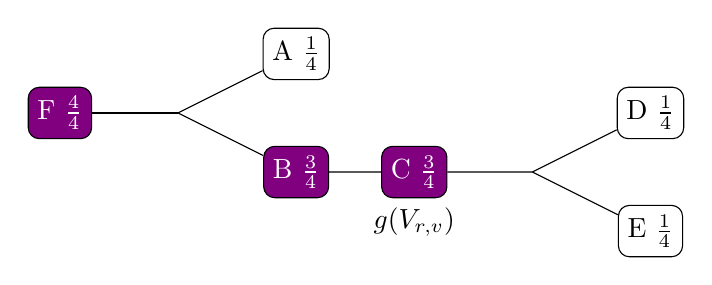
\begin{tikzpicture}[every node/.style = {shape=rectangle, rounded corners, draw, align=center}]
			\node [superprevote] {F $\frac{4}{4}$}
			child[grow=right] {
				child {
					node [superprevote] {B $\frac{3}{4}$}
					child {
						node [gprevote] {C $\frac{3}{4}$}
						child {
							child { node {E $\frac{1}{4}$} }
							child { node {D $\frac{1}{4}$} }
						}
					}
				}
				child { node {A $\frac{1}{4}$} }
			};
		\end{tikzpicture}
	}{}
\end{figure}

\subsubsection*{Example 2}

Consider a network split into two equally sized partitions.
Prevote messages are cast for $A$, $A$, $B$, $B$.
Since $F$ is on the branch of $A$ and $B$, it has a supermajority of votes even though no voter voted for it explicitly.
Importantly, notice that no new blocks are finalized because $F$ is already finalized.

\begin{figure}[H]
	\nemcenter{
		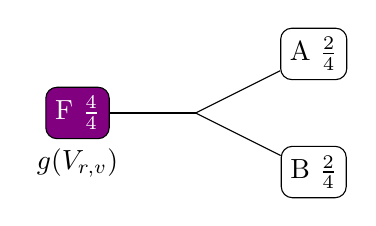
\begin{tikzpicture}[every node/.style = {shape=rectangle, rounded corners, draw, align=center}]
			\node [gprevote] {F $\frac{4}{4}$}
			child[grow=right] {
				child { node {B $\frac{2}{4}$} }
				child { node {A $\frac{2}{4}$} }
			};
		\end{tikzpicture}
	}{}
\end{figure}

\subsubsection*{Example 3a}

Prevote messages are cast for $A$, $B$, $C$, $D$ so that $B$ has a supermajority of prevotes.
Assume two voters see prevotes $A$, $B$, $C$ and send precommits for $A$.
Assume one voter sees prevotes $B$, $C$, $D$ and sends a precommit for $B$.
A voter can determine that the weight of unknown precommits (25\%) cannot cause a supermajority of precommits for $B$, which only has 25\% of precommits.
This satisfies condition 1 in \nemref{sec:finalization:algorithm}.

\begin{figure}[H]
	\nemcenter{
		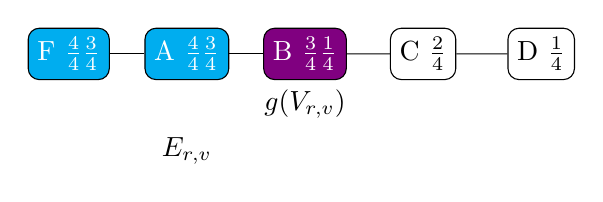
\begin{tikzpicture}[every node/.style = {shape=rectangle, rounded corners, draw, align=center}]
			\node [superprecommit] {F $\frac{4}{4}\frac{3}{4}$}
			child[grow=right] {
				node [superprecommit, gestimate] {A $\frac{4}{4}\frac{3}{4}$}
				child {
					node [gprevote] {B $\frac{3}{4}\frac{1}{4}$}
					child {
						node {C $\frac{2}{4}$}
						child {
							node {D $\frac{1}{4}$}
						}
					}
				}
			};
		\end{tikzpicture}
	}{}
\end{figure}

\subsubsection*{Example 3b}

Consider a slight modification of the previous example where prevotes are received in a different order.
As above, prevote messages are cast for $A$, $B$, $C$, $D$ so that $B$ has a supermajority of prevotes.
Assume two voters see prevotes $B$, $C$, $D$ and send precommits for $B$.
Assume one voter sees prevotes $A$, $B$, $C$ and sends a precommit for $A$.
A voter can determine that the weight of unknown precommits (25\%) cannot cause a supermajority of precommits for $C$, which only has 0\% of precommits.
This satisfies condition 2 in \nemref{sec:finalization:algorithm}.

\begin{figure}[H]
	\nemcenter{
		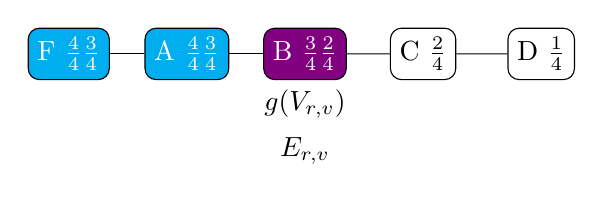
\begin{tikzpicture}[every node/.style = {shape=rectangle, rounded corners, draw, align=center}]
			\node [superprecommit] {F $\frac{4}{4}\frac{3}{4}$}
			child[grow=right] {
				node [superprecommit] {A $\frac{4}{4}\frac{3}{4}$}
				child {
					node [gprevote, gestimate] {B $\frac{3}{4}\frac{2}{4}$}
					child {
						node {C $\frac{2}{4}$}
						child {
							node {D $\frac{1}{4}$}
						}
					}
				}
			};
		\end{tikzpicture}
	}{}
\end{figure}

\subsubsection*{Example 4}

Consider an extension of the previous example where $A$ is committed at point $r-1$ but $B$ is not.
Now, the voters have moved to the next point $r$.
Four prevote messages and four precommit messages are cast for $F$.
Blocks $B$, $C$, $D$ have all been pruned from the main chain even though precommits for $B$ were used to commit $A$ at $r-1$.
In order to verify the proof at $r-1$, there needs to be a record that $B$ is a descendant of $A$.
This information is stored in the prevote message hash chains but not in the precommit messages.
This is why the verification of finalization proofs requires prevotes.

\begin{figure}[H]
	\nemcenter{
		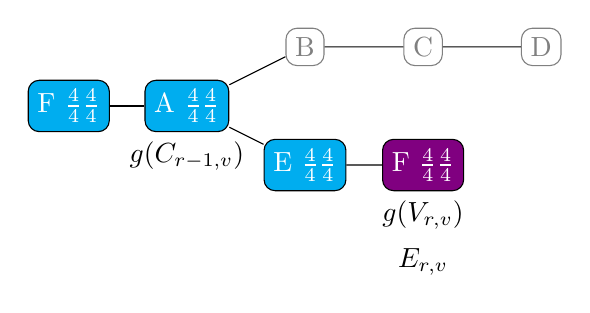
\begin{tikzpicture}[every node/.style = {shape=rectangle, rounded corners, draw, align=center}]
			\tikzset{ pruned/.style = {color=gray} }

			\node [superprecommit] {F $\frac{4}{4}\frac{4}{4}$}
			child[grow=right] {
				node [superprecommit, label=below:{$g(C_{r-1,v})$}] {A $\frac{4}{4}\frac{4}{4}$}
				child {
					node [superprecommit] {E $\frac{4}{4}\frac{4}{4}$}
					child {
						node [gprevote, gestimate] {F $\frac{4}{4}\frac{4}{4}$}
					}
				}
				child {
					node [pruned] {B}
					child {
						node [pruned] {C}
						child {
							node [pruned] {D}
						}
					}
				}
			};
		\end{tikzpicture}
	}{}
\end{figure}
